% Flowchart: Building Energy Prediction Pipeline
% Compile with pdflatex (requires TikZ, usually included in standard TeX)

\documentclass[11pt,a4paper]{article}
\usepackage[utf8]{inputenc}
\usepackage[T1]{fontenc}
\usepackage[margin=1in]{geometry}
\usepackage{tikz}
\usetikzlibrary{shapes.geometric, arrows.meta, positioning, fit, backgrounds}

\tikzset{
  startstop/.style={rectangle, rounded corners, minimum width=2.2cm, minimum height=0.6cm, draw=blue!60, fill=blue!10, align=center, font=\small},
  process/.style={rectangle, minimum width=2.2cm, minimum height=0.6cm, draw=orange!70, fill=orange!15, align=center, font=\small},
  decision/.style={diamond, minimum width=1.6cm, minimum height=0.5cm, draw=green!60!black, fill=green!10, align=center, font=\small},
  output/.style={rectangle, minimum width=2.2cm, minimum height=0.6cm, draw=teal!60, fill=teal!15, align=center, font=\small},
  app/.style={rectangle, rounded corners, minimum width=2.2cm, minimum height=0.6cm, draw=purple!60, fill=purple!10, align=center, font=\small},
  arrow/.style={-{Stealth[length=2mm]}, draw=gray!60, thick},
}

\begin{document}
\begin{center}
  \textbf{Metrik AI: Building Energy Prediction Pipeline} \\[0.3em]
  \small (Forecasting $\to$ Anomaly Detection $\to$ Decision Support $\to$ App)
\end{center}

\begin{figure}[h]
\centering
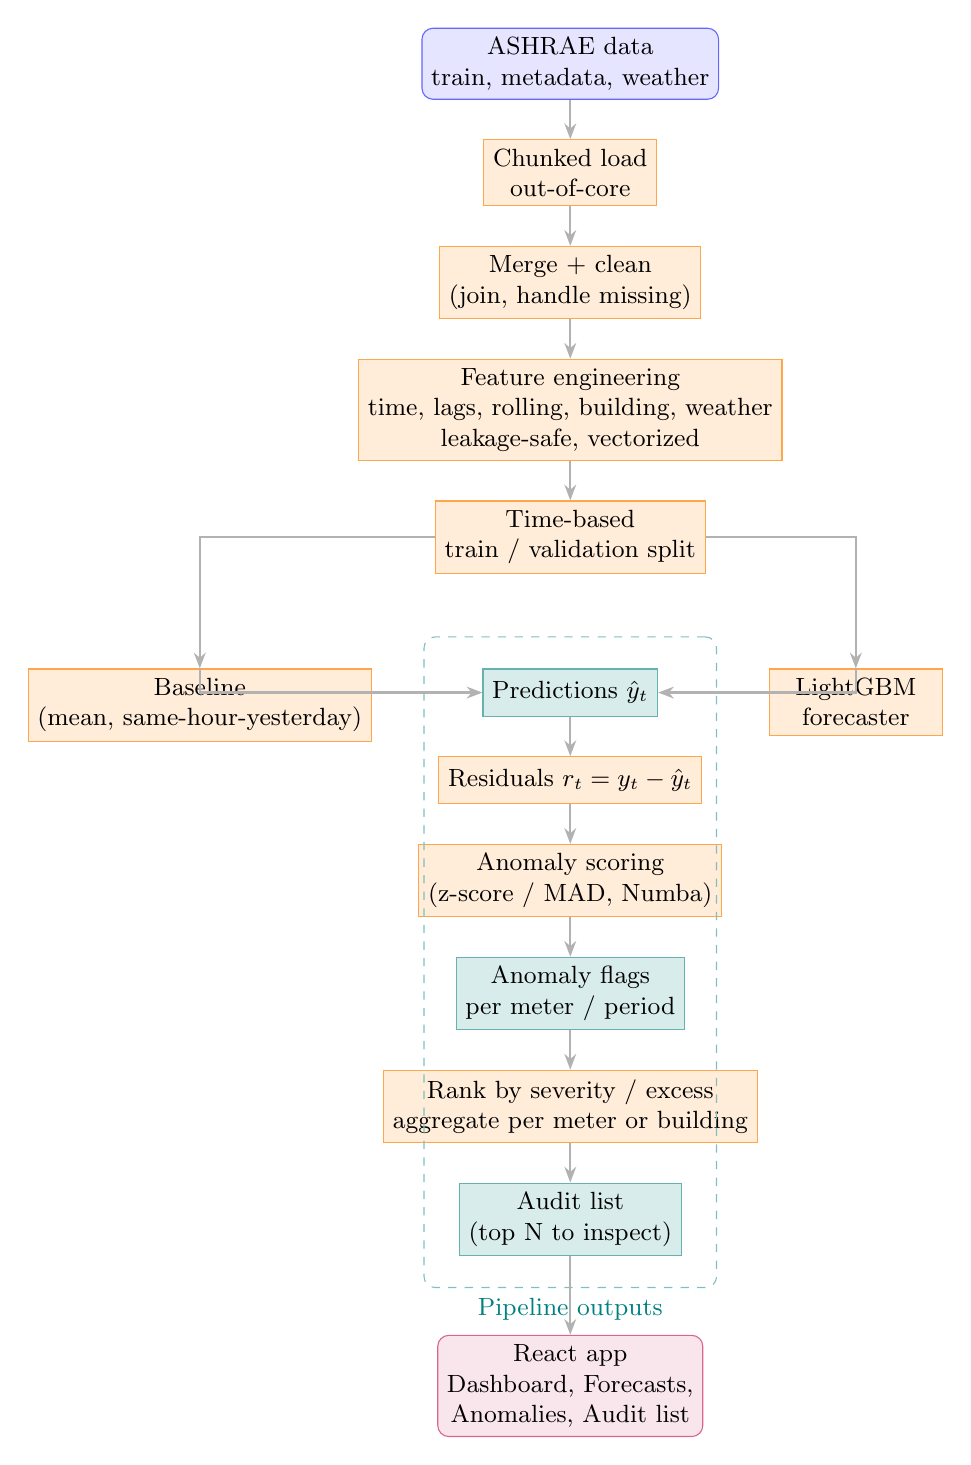
\begin{tikzpicture}[node distance=0.5cm and 0.8cm, every node/.style={font=\small}]

  % ---- Row 0: Data sources ----
  \node (data) [startstop] {ASHRAE data\\train, metadata, weather};

  % ---- Row 1: Load & clean ----
  \node (load) [process, below=of data] {Chunked load\\out-of-core};
  \node (merge) [process, below=of load] {Merge + clean\\(join, handle missing)};

  % ---- Row 2: Features ----
  \node (feat) [process, below=of merge] {Feature engineering\\time, lags, rolling, building, weather\\leakage-safe, vectorized};

  % ---- Row 3: Split ----
  \node (split) [process, below=of feat] {Time-based\\train / validation split};

  % ---- Row 4: Forecasting ----
  \node (baseline) [process, below left=1.2cm and 0.8cm of split] {Baseline\\(mean, same-hour-yesterday)};
  \node (lgbm) [process, below right=1.2cm and 0.8cm of split] {LightGBM\\forecaster};
  \node (preds) [output, below=1.2cm of split] {Predictions $\hat{y}_t$};

  % ---- Row 5: Anomaly ----
  \node (resid) [process, below=of preds] {Residuals $r_t = y_t - \hat{y}_t$};
  \node (score) [process, below=of resid] {Anomaly scoring\\(z-score / MAD, Numba)};
  \node (flags) [output, below=of score] {Anomaly flags\\per meter / period};

  % ---- Row 6: Decision support ----
  \node (rank) [process, below=of flags] {Rank by severity / excess\\aggregate per meter or building};
  \node (audit) [output, below=of rank] {Audit list\\(top N to inspect)};

  % ---- Row 7: Outputs box ----
  \node (outbox) [draw=teal!50, dashed, rounded corners, inner sep=0.4cm, fit=(preds)(flags)(audit), label={[teal]below:\small Pipeline outputs}]{};

  % ---- Row 8: React app ----
  \node (app) [app, below=1cm of audit] {React app\\Dashboard, Forecasts,\\Anomalies, Audit list};

  % ---- Arrows ----
  \draw [arrow] (data) -- (load);
  \draw [arrow] (load) -- (merge);
  \draw [arrow] (merge) -- (feat);
  \draw [arrow] (feat) -- (split);
  \draw [arrow] (split) -| (baseline);
  \draw [arrow] (split) -| (lgbm);
  \draw [arrow] (baseline) |- (preds);
  \draw [arrow] (lgbm) |- (preds);
  \draw [arrow] (preds) -- (resid);
  \draw [arrow] (resid) -- (score);
  \draw [arrow] (score) -- (flags);
  \draw [arrow] (flags) -- (rank);
  \draw [arrow] (rank) -- (audit);
  \draw [arrow] (audit) -- (app);

\end{tikzpicture}
\caption{End-to-end flow: raw data $\to$ chunked load and merge $\to$ leakage-safe features $\to$ time split $\to$ baseline + LightGBM $\to$ predictions $\to$ residuals $\to$ anomaly scoring $\to$ ranked audit list $\to$ React app.}
\end{figure}

\end{document}
